\documentclass[aip,amsmath, preprint, author-year]{revtex4-1}
\usepackage{url}
\usepackage[utf8]{inputenc}
\usepackage{hyperref}
\usepackage{graphicx} % for graphics
%\usepackage{listings} % for code listtings
%\usepackage{color}

%\setcitestyle{round, author-year}

\setcounter{page}{1}

%\bibliographystyle{aipauth4-1.bst}

\begin{document}

\begin{abstract}
An approach to generate generalised process capability data in order to populate and add functionality to a process capability database.
A description of the concept of generalisation, uses and implementation.
\end{abstract}

\title{Converting historical process capability into actionable robust design data - DRAFT}
\author{Andreas Bruun Okholm, s082562\\
Mathias Rask Møller, s082536 }
\affiliation{Technical University of Denmark}
 
\date{\today}
\maketitle

%Introduction

\section{Introduction}

All manufacturing process produces parts with variation of their specified dimensions.  
Understanding process variation and creating designs which are insensitive to the variation decreases cost of manufactured goods and increase user satisfaction. 
This is the main goals of the robust design methodology. 
Early research did focused on characterising the variation and understanding the related quality loss \cite{taguchi1986introduction}. 
During the 1990s many major american companies followed trend of robust design and created process capability databases (PCDB), however due the lack of practical tools for accessing process capability variation data these were largely unused for mechanical design purposes \cite{tata1999process}. 
While further research in PCDBs followed it still seems there is challenges needed to be solved before widespread adoption in industry is possible. 

In this paper we will do a literature review of PCDBs looking at both challenges and proposed solutions. 
We propose a modified indexing scheme for PCDBs and couple it with a new measure of process capability, which is easily understood and applicable for the the mechanical design engineer. 
This is one step to make it faster and easier for the mechanical designer to efficiently use process capability data in new designs. 

\section{Literature review}
There has been a significant amount of research, which shows use of process capability data (PCD) to set correct tolerances will reduce rework, cost, failure rate, assembly problems and improve product performance \citep{tata1999process}.

In the 90s several papers were published on methods to predict process variation using process models \citep{thornton2000use}. 
However creating process models can be very complicated and unpractical for many manufacturing process. 
Another option for acquiring process capability data is to measure the actual process performance and store it in a database. \cite{perzyk1998selection} describes such a database for storing general mechanical process capability data for the use of selecting optimal manufacturing methods.

Variance of a components dimension is usually the result of multiple processes. 
 \cite{kern2003forecasting} has developed a framework for a general process capability database that utilise a model of input and output variation of each (sub) manufacturing process. 

\subsection{Using Process Capability Data}
\cite{kern2003forecasting} identifies the following fields of study, where PCD is necessary for proper analysis: Design for Quality including Design for Six Sigma (DFSS), Quality Function Deployment (QFD), robust design, manufacturing variation modelling \& propagation, selective Assembly and tolerance allocation. 
Additionally Response Surface Methodology (RSM) and Statistical Process Control (SPC) does gather process data, which could be used in a PCD. 
The PCD is also necessary for the sub contractor to make qualified offers.


\subsection{Cost of manufacturing}
Including cost into the process capability database will make will make it possible to easily include the production price for the within design decisions \citep{perzyk1998selection, thornton2000use}. 
A general model for estimating the relationship between tolerance and price based on 5 different sources has been developed by \cite{sfantsikopoulos1990cost}.
It can be concluded that the relationship follows a simple general formula, but the parameter to relate tolerance to price for the specific manufacturing method needs to be estimated for every process. 

\subsection{Process capability databases in industry}
\cite{tata1999effective, tata1999process} found that major US companies within automotive, aerospace, military and consumer had created Process Capability Databases (PCDB) and were successfully using them for manufacturing control, but were unable to successfully utilise the PCDB for design. 
What hindered mechanical design from using PCD? 

\subsubsection{Key Challenges}
\textbf{Fragmented Organisation.}  A PCDB is a cross departments part form usually involving manufacturing, quality control and mechanical design within the company. 
Creating a project which meets the interests of all department is challenging. 
Managers does not fully understand the need for a PCDB and the resources required to collect and analyse the information. 
Lack of company wide visions for the PCDB results in locally developed and maintained within a particular manufacturing location or departments. 
The use of PCD in design projects is not directly encouraged and rewarded. 

\textbf{Data Comunication.} Creating efficient indexing systems that allows for unambiguous process, feature geometry, material and stock selection. 
The databases are typically not easily searchable which makes it very difficult to find the correct data and in many cases the data sought after data does not exists. 
The data is not presented in a way which is easily understandable by mechanical designers.

\textbf{Information Technology.} Creating a database thats globally accessible and accept inputs from multiple different clients and interface with existing systems is complex.
Developing the indexing systems and user interface for multiple different uses cases is also resource demanding task.  

\subsubsection{Proposed Solutions}
In the book "Variation Risk Management" \cite{thornton2004variation} presents a variety variation management strategies to be used in a company. 
Key Characteristics (KC) can be a product, system, assembly, part or process characteristics for which the cost of variation is high and the variation is high. 
KC's should have most focus for optimal use of resources. 

It is individual for different companies what data should be stored in a PCDB, but a general list consist of material, stock, process, feature dimension, lower limit, upper limit, machine, operator number, batch size, mean, standard deviation for each record. 
Each record is a summation of multiple measurements made of a batch of parts \citep{thornton2004variation}.

Using graph theory a graphical display for manufacturing capability is developed, which provides quick overview \citep{thornton2000use}. 
One of the key views shows bias of a set of measurements along the horizontal axis and the standard deviation of the measurement set along the vertical axis. 
Confidence intervals in both bias and std. are shown for each measurement to visualise the statistical significance. 
A systems for automatically detecting and visualising trends in the data is also described.

\cite{kern2003forecasting} recognised that the success of the system relies on consistent and correct data input. 
A method to index design characteristics is developed to consistently assign correct key features on parts. 
Being one of the most elaborate works on PCDB the target seems to highly specialised productions companies. 


\subsection{Public Process Capability Data}
From our own search we haven't been able to find any public available process capability database. 
We have searched using Google, Google scholar and DTU library, using the search words: "process capability database", "Example process capability", "open process database", "Process variance database", "variance prediction database", "process variance table" without success. 

There exists some very general guide tables relating tolerance grade (IT-scale) and machining operation \citep{united1967preferred, american1978preferred}. 
It is however unclear how the data for the table has been generated.

In \cite[p. 715]{oberg2008machinery} there is given a figure showing the surface roughness from common production methods. From 50 Ra to 0.012. 
Again no source of the information is given. \\[1cm]

\section{Easy to use actionable Process capability database }
In this article we present a concept of data indexing, processing and presentation which tries to make it faster and easier for the mechanical designer to efficiently use process capability data in new designs. 
The general principle is to provide an interface where the data is presented in a much more generalised than typically done in PCDB interfaces. 
The core indexing scheme is simplified, but details are retained or improved using a flexible tagging system. 
Instead of presenting the designer with statistical information, recommended specifications limits based on actual PC is shown directly. 
The specification limits is normalised in regard to the specified dimension making more use out of each dataset, minimising the risk of PC requests not returning any results. 

Combined with advances in information technology we hope this will help make PCDBs a viable tool in the mechanical design process. 

\subsection{Indexing}

\begingroup
\squeezetable

\begin{table*}
\begin{ruledtabular}
\caption{\label{tab:sampleset} Measurement set - As stored in the PCDB}
\begin{tabular}{lllllllll}
\textbf{Material*} 		& \textbf{Process*} 		& \textbf{Meas. Equipment}  	& \textbf{Target*} 	& \textbf{LSL} 	& \textbf{USL} 	& \textbf{Mean Shift*} 	& \textbf{Std.}   $\hat{\sigma}$ * & 	\\
Thermoplastic 			& Moulding			& CT Scanning				& 3.00			& 2.99		& 3.01		& -0.0486			& 0.0032				\\
 - ABS, PC blend		& - Injection Mould.		& Zeiss metrotom 800	\\
\\
\textbf{General Tag (1)} 	& \textbf{General Tag (2)} & \textbf{General Tag (3)} 	& \textbf{Geometry}		& \textbf{Measurement Date} 	& \textbf{N samples} 	\\
Mould Type			& Product color			& Production run			& Diameter				& 13 oct. 2013  			& 12\\
- Steel 				& - Red				& - PR3				\\
- - NAK80 
\end{tabular}%
\end{ruledtabular}
\end{table*}
\endgroup


PCDBs needs to be indexed to efficiently retrieve data of relevance to the current design. 
The data stored in a PCDB is typically measurement sets; the statistical result of a number of measurements from a given part dimension combined with the design characteristics (DC). 
Feature, geometry, material and process is suggested by \cite{kern2003forecasting} to be the primary DCs. 
For each primary DC there exists a tree structure of possibilities. An example of an index using Kerns proposed design index could be "Plane", "Position", "Aluminium", "Turning" as feature, geometry, material and process respectively. 

We propose to use \emph{material} and \emph{process} as the only required DCs. 
\emph{Geometry} information: distance, radius, diameter or positions is readily available from the measurement tool and should be stored as well, but not necessarily used when querying the database.
This is combined with a \emph{tagging system}, where additional tags can be inputted. 
Common tags can be selected from tree structure. 
Tags gives flexibility since more than one tag can be applied to one measurement set and it is possible to index for DCs that are specific to a single production method or material. 

Example: For injection moulding it would be interesting to index the following DCs:
\begin{itemize}
\item Material type of the mould: aluminium, steel, hardened, etc.
\item Mould/Process iterations (T0, T1, T2, ...) could also give valuable insights of which specification limits requires mould rework or process adjustment. 
\item Tagging dimensions measured a crosses parting lines could potentially showing a general increase in desired specification limits.
\end{itemize}
It would not be possible to index these DCs, which are specific for the process without having optional tags. 
A complete database record of a sample set can be seen in table \ref{tab:sampleset} showing all data connected to the sampleset. 

\emph{No feature index:}
In casting and injection moulding, two of the most used processes for mass produced part, feature is not necessarily an important DC. 
The individual features are manufactured by the same computer-aided manufacturing (CAM) milling machine with the same process parameters. 
For features with properties such as high length to width ratios could be optionally tagged. 
In a fully integrated robust design process interaction between components are reduced to as small and simple surfaces as possible further reducing the need for a features index.

\subsection{Processing Capability Data}

Processing the capability data consists of three steps: 

\begin{enumerate}
	\item Compute the process capability specification limit (PCSL) - the required specification limits (tolerance) to achieve a desired performance using the given process capability.
	\item Normalise the PCSLs so it is independent of dimension.
	\item Fit operating curves to the PCSL data grouped by different design characteristics.
\end{enumerate}

\subsubsection{Process Capability Specification Limit}
The process capability indices ($C_p$ and $C_{pk}$) described by \cite{kane1986process} has been widely adopted in statistical process control, been extended and further researched for better understanding \citep{wu2009overview}. 
Instead of looking at process mean $\mu$, standard deviation $\sigma$ and specification upper and lower limits $USL$, $LSL$ using process capabilities indices (PCIs) transforms these values into unit less numbers, which provides a quick overview of how a process is performing.

The PCIs ability to transform process variables of any object into unit less capability index can be reversed to calculate desirable specification limits. For en example the commonly used PCI $C_{pk}$ 
\begin{equation}
	C_{pk} = \frac{d - | \mu - m|}{3 \sigma} \nonumber
\end{equation}
can be reversed
\begin{equation}
	d = 3 C_{pk} \sigma + | \mu - m|
\end{equation}
Where $d = (USL - LSL) / 2$ is half the specification limit and $m = (USL + LSL) / 2$ is the midpoint between the specification limits. When $d$ is reversely used to estimated the required tolerance to achieve the desired process capability index value we call this the process capability specification limit (PCSL). 

Using the data from table \ref{tab:sampleset} and a $C_{pk} = 1.66$. The PCSL is computed: 
\begin{align*}
PCSL &= 3 \cdot 1.66 \cdot 0.0032 \, \mathrm{mm}
+ |0.0486  \, \mathrm{mm}| \\
&= 0.0645  \, \mathrm{mm}
\end{align*}


There are several commonly used PCIs each serving their purpose \citep{wu2009overview, taguchi1986introduction}
\begin{itemize}
	\item $C_a$ : Closeness of process mean to target 
	\item $C_p$ : Relative size of variation
	\item $C_{pk}$ : Amount of nonconforming (\%NC)
	\item $C_{pm}$ : Value loss (Taguchi loss function)
	\item $C_{pmk}$: Version of $C_{pm}$,  sensitive to mean shift. 
\end{itemize}

Visualising the $CPIs = 1$  shows how a process on target $C_a = 1$ allows the same variation for all PCIs see figure \ref{fig:CPI}. 
The line for $C_{pm}$ is in below that of $C_{pk}$ except for values of $C_a$ close to 1. 
Using $C_{pm}$ will in general be more conservative resulting in larger specification limits than $C_{pk}$. The plot shown is for a capability equal to one for higher values this effect is even more pronounced.

\begin{figure}
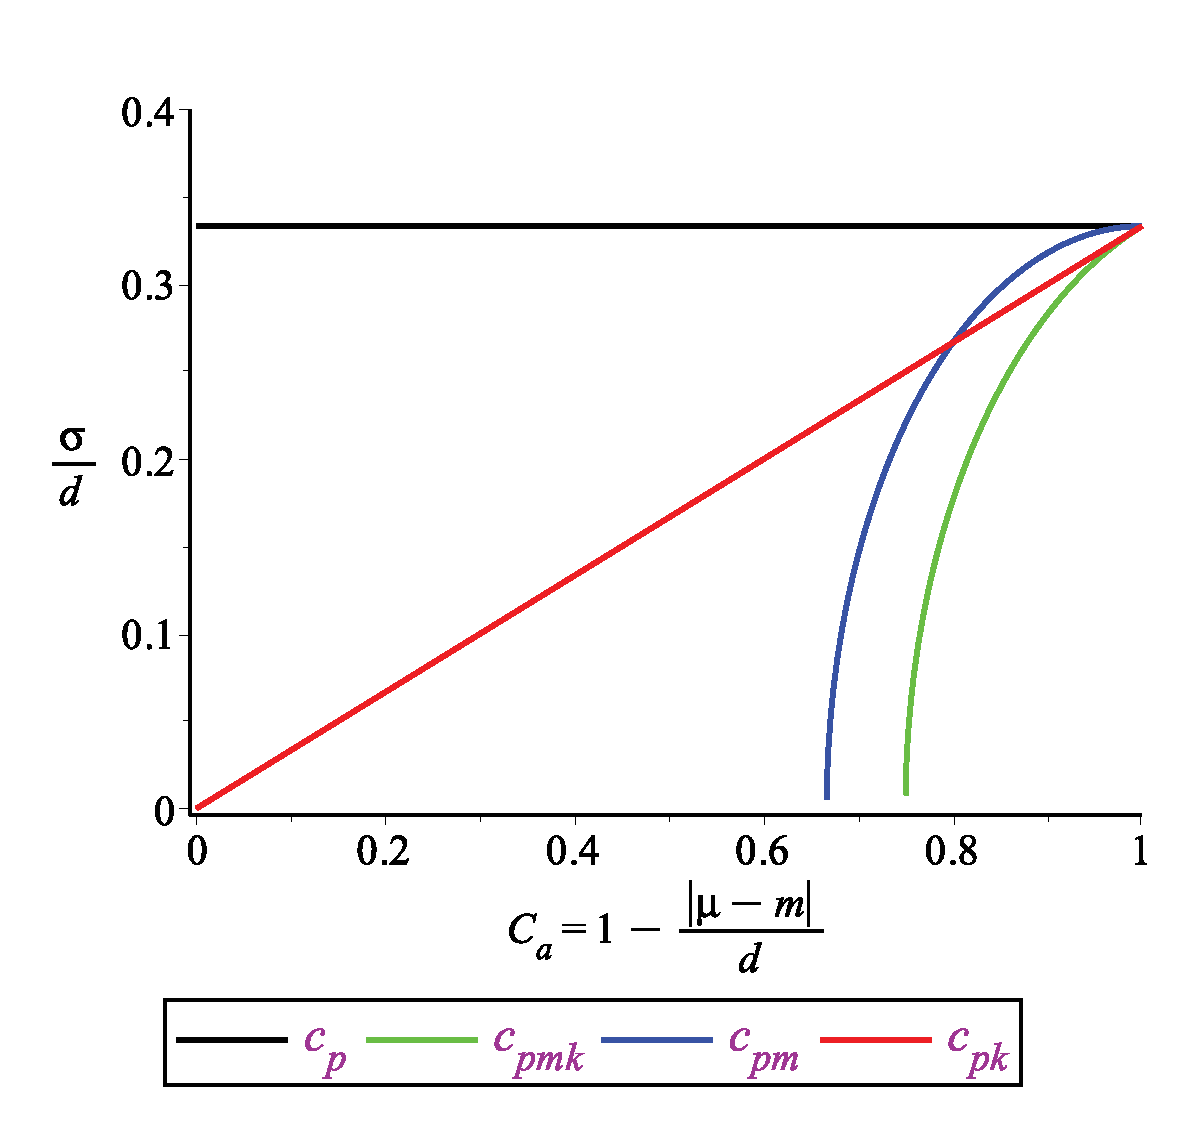
\includegraphics[width=0.45\textwidth]{graph_postscript_test.eps}
\caption{\label{fig:CPI} Nomalised standard deviation as a function of normalised meanshift. $C_p$ referens only to the variance of the process. 
$C_{pk}$ is related to the yield of the product. $C_{pm}$ takes a loss function in to account relates to a target dimension. 
$C_{pmk}$ takes both the yield of the product and a loss function. }
\end{figure}

For the purpose of our database we have chosen to use $C_{pk}$, since it provides the most easily understandable result - directly related to the yield of the process. The yield of a process is within
\begin{equation}
	2\Phi(3C_{pk})-1 \leq \text{yield} < \Phi(3C_{pk}) \nonumber
\end{equation}

where $\Phi(\cdot)$ is the cumulative distribution function of the standard normal distribution N(0,1) \citep{boyles1991taguchi}. 
For typical capability levels the resulting non-conforming products in parts per million (ppm) is listed in table \ref{tab:cpl_nc}

\begin{table}
\begin{ruledtabular}
\caption{\label{tab:cpl_nc} $C_{pk}$ Non-conformities}
\begin{tabular}{llll}
  $\mathbf{C}_{pk}$	& $\sigma$ level	& $\mathbf{NC_\mathrm{max}} \mathrm{\ (ppm)}$	&  $\mathbf{NC_\mathrm{min}} \mathrm{\ (ppm)}$	\\
  1.00	& 3		& 2699.8		& 1349.9		\\
  1.33 	& 4 		& 63.3		& 31.7 		\\
  1.50 	& 4.5 	& 6.7		& 3.4		\\
  1.66	& 5		& 0.6		& 0.3		\\
  2.00	& 6		& 0.002		& 0.001		\\
\end{tabular}%
\end{ruledtabular}
\end{table}

The optimal process capability index value depends on the application, however there exists a practice in quality control called six sigma $(6 \sigma)$, which advocates the use of six sigma ($C_{pk} = 2$) for short term process capability will generally improve manufacturing quality and profits \cite{koch2004design}. 

It's assumed that the process drifts over time up to $1.5 \sigma$  (effectively resulting in a sigma level of 4.5), which still results in an acceptable 3.4 ppm defects.
For the PCSL to reflect six sigma production capability the $C_{pk}$ input with each measurement set should be varied from 2.0 to 1.5 $C_{pk}$ depending wether the measurement set reflects the short or long term capability. 
For simplicity we propose to use a value general value of $C_{pk} = 1.66$ to account for a  mixture of long term and short term measurements. 

We have focused on $C_{pk}$ through most of this section.
In situations where the desired tolerances directly influence product performance, for instance in lens optics construction, using the more abstract $C_{pm}$ might make more sense. 


\subsubsection{Normalization}
The calculated Process Capability Specification Limits (PCSL) are normalised so it can be used to predict PCSLs for any dimension within the limit of the normalisation algorithm. 
This reduces the required amount of data in the database before it's useful for mechanical design since it is possible to use PC information from components of different sizes.

There exists industrial standards used for manufacturing which describe the "normal" relationships between linear dimensions and tolerances. 
We have analysed the most commonly used standards for general tolerances: American \citeauthor{american1978preferred}, European \citeauthor{ISO286} and the German \citeauthor{DIN7168}. 
The ANSI and the ISO standards uses the same formula and are quite close to the german DIN standard. 
These standards display a non-linear relationship between tolerance and dimension. 
For the same level for precision, the tolerances of large dimensions are smaller relatively than for small dimensions. See figure \ref{fig:tolstd}.

The German \citeauthor{DIN16901} and the French \citeauthor{NFT58000} are standards specifically for moulded plastic parts. 
These standards present an almost linear relationship between tolerance and dimension. 
This might be due that a major contributing error in moulded parts is a result of creep, since creep errors in general has a linear relationship between overall dimension and error.

\begin{figure}
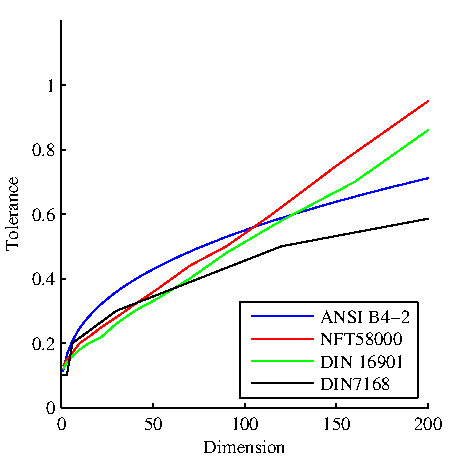
\includegraphics[width=0.5\textwidth]{Tolerance_standards.pdf}
\caption{\label{fig:tolstd} \citeauthor{DIN16901} (POM 120) and \citeauthor{NFT58000} (normal) are standards specifically for moulded plastic components. They are almost linear for sizes above 10 mm. 
\citeauthor{american1978preferred} (gr. 13) and \citeauthor{DIN7168} (medium) describes a general relationship between linear tolerances and dimension. All standards included several levels of precission.}
\end{figure}

These standards are all described using a tables showing the tolerances for a given dimension intervals and precision. 
In a note for \citeauthor{american1978preferred} and later mentioned in \citeauthor{ISO286} a continuous function is described for IT-grades (precision levels) between IT6 to IT16 for dimensions from 2 mm to 500 mm. 
This function is for unknown reasons not included in newer versions of ISO 286 yet table values seems still estimated using this function.

\begin{align}
	T =& 10^{0.2 (ITG -1)} \cdot i \\
	i =& 0.45 \sqrt[3]{D} + 10^{-3} \, D 
\end{align}

Where $i$ is standard tolerance factor, $D$ is the nominal mean dimension $D = \sqrt{D_{\textrm{min}} D_\textrm{max}}$ in $[mm]$ and $T $ is the tolerance width in $[\mu m]$ , which is equal to $2d$. 

In the generalised PCDB the measurement sets PCSL are normalised using said function because ISO 286 is general practice in the industry. 
Further work on improving the normalisation feature requires more data than what is available to us. Normalization actual data for the different processes.

The IT-grade for the measurement set presented in table \ref{tab:sampleset} can be computed.

\begin{align*}
&\mathrm{ITG} = 5 \cdot \log_{10} \left\{ \frac{T \cdot 10^3}{ 0.45  D^{\frac{1}{3}} + D \cdot10^{-3} }\right\} +1 \\
&\mathrm{ITG_{spec} }= 13.4 \\
&\mathrm{ITG_{actual}} = 12.5
\end{align*}

The $\mathrm{ITG_{actual}}$ is based on the measurements  and is calculated using $T = 2 \, PCSL$ and the $\mathrm{ITG_{spec}}$ is specified by the design and is calculated using $T = 2 \,USL$ for symmetric tolerances. 

\subsubsection{Analyze normalized data}
A further analysis of the underlying measurements sets is done to present the user with a easier to use data view. 
Relevant measurements sets are aggregated based on DC's selected by the user. 

To help the user determine which tolerance to use, a accumulated frequency plot of the normalised PCSL is proposed. 
This gives an overview of the current process capability assuming it has not changed since the data has been recorded. 
The plot shows the probability, if production capability were randomly selected, to produced the selected part at a specified $C_{pk}$ and tolerance, see figure \ref{fig:acumfreq}. 
A normal distribution is fitted to the data to show a continuous function.

Selecting a tolerance associated with a low probability will generally impact the price of production since it either: 
Increases risks of rework to hit the target $C_{pk}$ or requires more precise machines than what is used for the measured components.

\begin{figure}
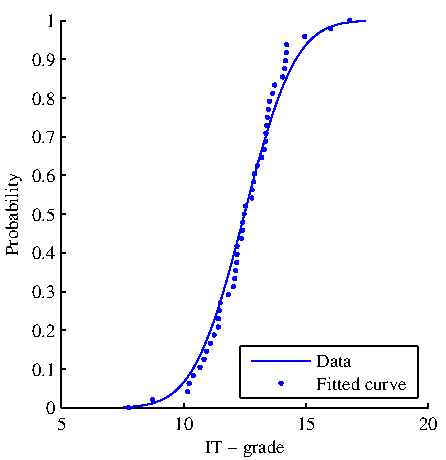
\includegraphics{Acum_freqIT.pdf}
\caption{\label{fig:acumfreq} Accumulated frequency IT grade distribution, $C_{pk} =1.66$. 
20 measurement sets each containing between 3 and 219 samples. 
Actual data from \cite{thornton2000use}. }
\end{figure}

It is possible to easily compare multiple CDs by displaying them in the same view. In figure \ref{fig:acumfreqF3} PC data from two machines is shown respectively. 
It is possible to see that the machine marked '1031' performs better than '1032', but '1032' is more consistent.

\begin{figure}
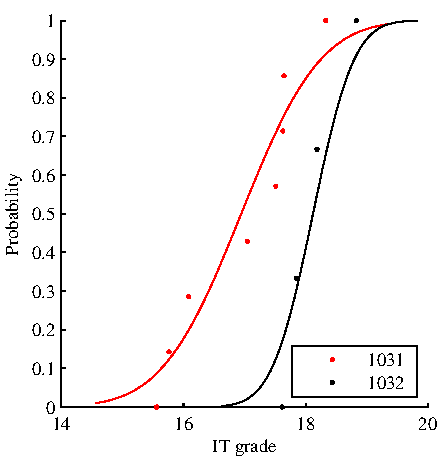
\includegraphics{Acum_freqF3.pdf}
\caption{\label{fig:acumfreqF3} Comparing two differnet DC's. 
Measurement sets from machine nr. 1031 and 1032 respecfully. 
Accumulated frequency IT grade distribution, $C_{pk} =1.66$. 
Actual data from \cite{thornton2000use}. }
\end{figure}

Further consideration are done in order display the information in a more comprehensible way.
\begin{itemize}
\item The tolerance can be shown in $[mm]$ instead of IT-grade for a user selected dimension.
\item In a web environment a popup activated by hover interactivity allow the user to see specifics of each data point.
\item Confidence limits for the estimated distribution should be shown to ensure statistically validity.
\end{itemize}

\subsection{Statistical Validity}
The user needs to trust the information provided by the PCDB. 
The uncertainty of the resulting distribution of IT grades is influenced by several factors.
\begin{itemize}
\item More samples in each measurement set will increase certainty. 
\item More measurements sets increases the certainty. 
\item Lower standard deviation of the IT grade distribution will increase the certainty.
\item Higher mean deviations from target $C_a$ will slightly increase the certainty especially at low sample sizes.
\end{itemize}
Sample size and number of measurement sets are the only two possible actionable variables. 

\subsubsection{Monte Carlo simulaiton}
To model the uncertainty and accuracy of the IT-grade distribution we have chosen to use Monte Carlo simulation, since it would be very difficult to accurately model analytically. 
We assume that the IT-grade (ITG) from each measurement set is continuous random variate with mean $\mu_{\mathrm{ITG}}$ and standard deviation $\sigma_{\mathrm{ITG}}$ giving $\mathrm{ITG} \sim \mathcal{N} (\mu_{\mathrm{ITG}}, \sigma_{\mathrm{ITG}}^2)$

The randomly generated ITG is converted into a normal distribution of individual measurements X using a fixed target dimension of $m = 100 \mathrm{\ [mm]}$ and closeness to target $C_a = 0.6$. 
The standard deviation $\sigma_{X}$ and mean shift $| \mu - m|$ can be calculated yielding the distribution parameters $\mathrm{X} \sim \mathcal{N} (| \mu - m|, {\mu_{\mathrm{X}}}^2)$. 

Each measurement is generated from the measurement set distribution.
When all measurements has been generated the process is reversed and the distribution parameters of ITG is estimated.
The simulation is run $N$ times.

Using the Monte Carlo simulation found that the standard deviation of the IT grade distribution is overestimated especially at lower sample sizes dues the increased uncertainty of these. 
Even at sample sizes of 10 it's still overestimated by 10 \%. 
This effect can be seen on figure \ref{fig:confidenceIntervals}. The mean value is within 1 \% of the original value and is independent of sample size and number of measurements.  

\begin{figure}
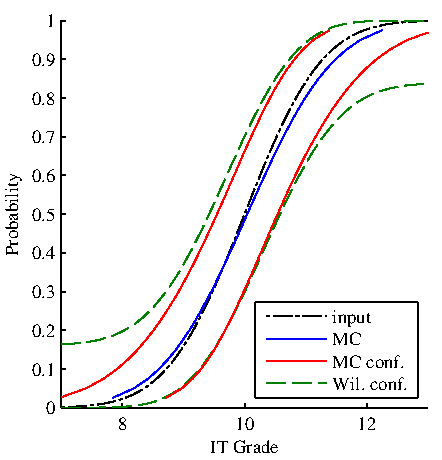
\includegraphics{confidenceIntervals.pdf}
\caption{\label{fig:confidenceIntervals}Cummulated frequency plot showing the input distribution of IT-grade $\mathrm{ITG} \sim \mathcal{N} (10, 1)$. 
The Monte Carlo simulation were run $N = 10,000$ times. 
The 95\% confidence intervals estimated by the Monte Carlo is simelar to the Wilson score in the center in the part of the probability distribution.}
\end{figure}

The Monte Carlo simulation were also used to estimated the confidence intervals at different cumulative probabilities using the percentile method.
The percentile method interval is the interval between the $100 \cdot \alpha$ and $100 \cdot (1-\alpha)$ percentiles of the Monte Carlo distribution. 

To verify the simulation we compared the confidence intervals to a simple approximation of the interval based on the Wilson score interval for the same input at the Monte Carlo, as can be seen in Figure \ref{fig:confidenceIntervals}. The Monte Carlo interval width is very close to the wilson score at midsection of probability curve. 
The confidence intervals for the Wilson score deviates at the top and bottom section which is a property of the wilson approximation.

The effects of sample size and number of measurements sets is displayed in Figure \ref{CLW90_lines.pdf} which shows the confidence interval width at a cumulative probability of 90 \% as a function of sample size and number of measurement sets. 
Increasing sample size only have an effect up to about 12 samples, additional sample measurements does not increase accuracy. 
The amount of measurements sets is the main factor for reducing the confidence intervals. 
If the purpose is too differentiate between DCs then the number of measurements sets is going to limit how small the differences between DCs can be resolved with statistical certainty.

\begin{figure}
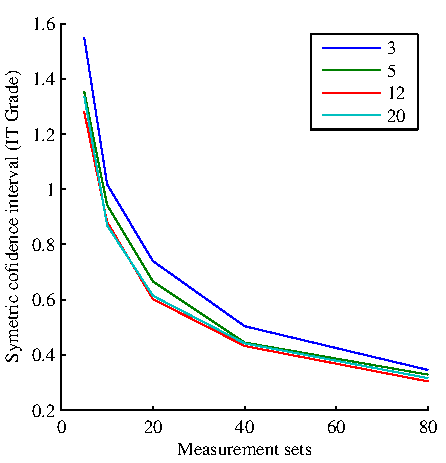
\includegraphics{CLW90_lines.pdf}
\caption{\label{fig:cl_line} Monte Carlo simulation of the cofidence interval width as a function of both sample size and number of measurement sets. 
Confidence interval width is measured in IT-grades. 
The number of sample sets has much bigger influence than sample size for sizes above 12 samples.}
\end{figure}



\section{Insights from }


The effect of a low sample size is shown in figure \ref{fig:effect}. 
The standard deviation of the deviation is overestimated compared the input distribution.

\section*{References}
\bibliography{../PCDBmasterBibliography/PCDB_Master_bib.bib}

\end{document}